\clearpage
%
% PART II: FRAME BENCHMARKS
%
% Make listings font size smaller for input and output files
\lstset{basicstyle=\ttfamily\scriptsize, columns=fullflexible, keepspaces=true}
%
% FRAME TYPE: I
%
\subsection{One-Bay, One-Storey Frame with Pin and Roller Supports and a Tie Member}
The first frame to be analyzed under three different load cases is demonstrated in the figure 
below. It will be referred to as FR1 in the following parts.
\begin{figure}[h]
    \includegraphics[scale=0.75]{%
                            bm_figures/turtle_figures/bmfr_FR1_turtle.pdf}
    \centering
    \caption{Frame FR1}
    \label{fig:bmfr01_turtle}
\end{figure}
\par
Three different cross sections are assigned to the four members that the frame is composed of,
and the areas are amplified by a factor of $10^7 I_i/l_i^2$ to mimic axial rigidity by ensuring
that the axial stiffness is orders of magnitude greater than the bending stiffness for each
member. Cross sectional properties of each member are summarized via the following table:
\begin{table}[h!]
\centering
\begin{tabular}{ c c c c c c}
    Member & b(m) & h(m) & I($m^4$)    & l(m) & A($m^2$)       \\ \hline \\
    AB     & 0.3  & 0.6  & 0.54000E-02 & 6.0  & 0.15000000E+04 \\
    BC     & 0.3  & 0.5  & 0.31250E-02 & 8.0  & 0.48828125E+03 \\
    CD     & 0.3  & 0.6  & 0.54000E-02 & 6.0  & 0.15000000E+04 \\
    AD     & 0.3  & 0.3  & 0.67500E-03 & 8.0  & 0.10546875E+03 \\
\end{tabular}
\end{table}
\par
To ease the process of parametric analysis, some factors are used which take the different cross 
sectional properties into account. These factors are used in the parts to come to compute
the analytical values of the desired quantities, and therefore presented below for the sake of
completeness.
\begin{table}[h!]
\centering
\begin{tabular}{ c c c }
    Factor   & Expression & Value       \\ \hline \\
    $k_1$    & $\dfrac{I_{BC}}{I_{AD}}$                 & 4.62963  \\
    $k_2$    & $\dfrac{I_{BC}}{I_{AB}}\dfrac{h}{l}$     & 0.43403  \\
    $R_1$    & $2k_2+3$                                 & 3.86806  \\
    $R_2$    & $3k_1+2k_2$                              & 14.75694 \\
    $F_1$    & $R_1R_2 - k_2^2$                         & 56.89230 \\
    $F_2$    & $1+k_1+6k_2$                             & 8.23380  \\
\end{tabular}
\end{table}


%
% LOAD CASE 1
%
\subsubsection{Load Case 1}
\begin{figure}[h]
    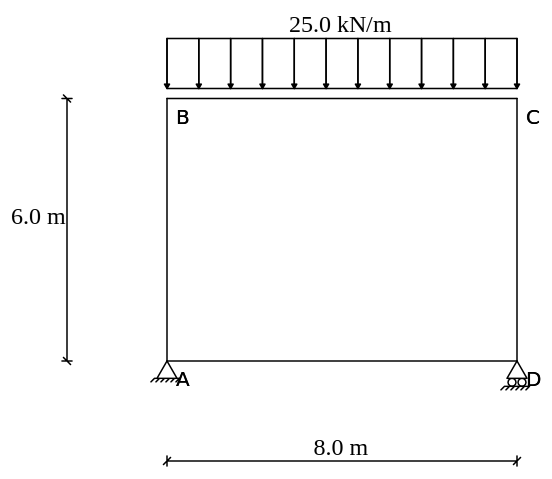
\includegraphics[scale=0.75]{%
                            bm_figures/turtle_figures/bmfr01_turtle.pdf}
    \centering
    \caption{Problem 1: Loading, geometry and supports}
    \label{fig:bmfr01_turtle}
\end{figure}
\lstinputlisting{input_files/bmfr01_input.dat}
\lstinputlisting{output_files/bmfr01_output.dat}
% Deformed
\begin{figure}[!htb]
    \includegraphics[width=\textwidth, keepaspectratio]{%
                     bm_figures/vtk_figures/bmfr01_deformed.pdf}
    \centering
    \caption{FR1, Load Case 1: Deformed Shape}
    \label{fig:bmfr01_deformed}
\end{figure}
% Axial
\begin{figure}[!htb]
    \includegraphics[width=\textwidth, keepaspectratio]{%
                     bm_figures/vtk_figures/bmfr01_axial.pdf}
    \centering
    \caption{FR1, Load Case 1: Axial Force Diagram}
    \label{fig:bmfr01_shear}
\end{figure}
% Shear
\begin{figure}[!htb]
    \includegraphics[width=\textwidth, keepaspectratio]{%
                     bm_figures/vtk_figures/bmfr01_shear.pdf}
    \centering
    \caption{FR1, Load Case 1: Shear Force Diagram}
    \label{fig:bmfr01_shear}
\end{figure}
% Moment
\begin{figure}[!htb]
    \includegraphics[width=\textwidth, keepaspectratio]{%
                     bm_figures/vtk_figures/bmfr01_moment.pdf}
    \centering
    \caption{FR1, Load Case 1: Bending Moment Diagram}
    \label{fig:bmfr01_moment}
\end{figure}
% Error
\begin{table}[h!]
\centering
\begin{tabular}{ c| c c c c }
    & Exact Expression & Exact Value & Computed Value & \% RE \\ \hline \\
    $M_A=M_D$   & $\dfrac{\omega l^2}{4}\dfrac{k_2}{F_1}$ &  0.30516E+01 & 0.30516E+01 & 0.0\% \\ \\
    $M_B=M_C$   & $\dfrac{-\omega l^2}{4}\dfrac{R_2}{F_1}$ &  -0.10375E+02 & -0.10375E+02 & 0.0\% \\ \\
    $M_{max}$   & $\dfrac{\omega l^2}{8} + M_B$ &  0.96246E+02 & 0.96247E+02 & 0.001\% \\ \\
    $V_A=V_D$   & $\dfrac{\omega l}{2}$ &  0.10000E+03 & 0.10000E+03 & 0.0\% \\ \\
\end{tabular}
\end{table}

%
% LOAD CASE 2
%
\clearpage
\subsubsection{Load Case 2}
\begin{figure}[h]
    \includegraphics[scale=0.75]{%
                            bm_figures/turtle_figures/bmfr02_turtle.pdf}
    \centering
    \caption{Problem 1: Loading, geometry and supports}
    \label{fig:bmfr02_turtle}
\end{figure}
\lstinputlisting{input_files/bmfr02_input.dat}
\lstinputlisting{output_files/bmfr02_output.dat}
% Deformed
\begin{figure}[!htb]
    \includegraphics[width=\textwidth, keepaspectratio]{%
                     bm_figures/vtk_figures/bmfr02_deformed.pdf}
    \centering
    \caption{FR1, Load Case 2: Deformed Shape}
    \label{fig:bmfr02_deformed}
\end{figure}
% Axial
\begin{figure}[!htb]
    \includegraphics[width=\textwidth, keepaspectratio]{%
                     bm_figures/vtk_figures/bmfr02_axial.pdf}
    \centering
    \caption{FR1, Load Case 2: Axial Force Diagram}
    \label{fig:bmfr02_shear}
\end{figure}
% Shear
\begin{figure}[!htb]
    \includegraphics[width=\textwidth, keepaspectratio]{%
                     bm_figures/vtk_figures/bmfr02_shear.pdf}
    \centering
    \caption{FR1, Load Case 2: Shear Force Diagram}
    \label{fig:bmfr02_shear}
\end{figure}
% Moment
\begin{figure}[!htb]
    \includegraphics[width=\textwidth, keepaspectratio]{%
                     bm_figures/vtk_figures/bmfr02_moment.pdf}
    \centering
    \caption{FR1, Load Case 2: Bending Moment Diagram}
    \label{fig:bmfr02_moment}
\end{figure}
% Error
\begin{table}[h!]
\centering
\begin{tabular}{ c| c c c c }
    & Exact Expression & Exact Value & Computed Value & \% RE \\ \hline \\
    $M_A=M_D$   & $\dfrac{3}{8}Pl\dfrac{k_2}{F_1}$ &  0.11443E+01 & 0.11443E+01 & 0.0\% \\ \\
    $M_B=M_C$   & $\dfrac{-\omega l^2}{4}\dfrac{R_2}{F_1}$ &  -0.38908E+02 & -0.38908E+02 & 0.0\% \\ \\
    $M_{max}$   & $\dfrac{pl}{4} + M_B$ &  0.61092E+02 & 0.61092E+02 & 0.0\% \\ \\
    $V_A=V_D$   & $\dfrac{P}{2}$ &  0.25000E+02 & 0.25000E+02 & 0.0\% \\ \\
\end{tabular}
\end{table}

%
% LOAD CASE 3
%
\clearpage
\subsubsection{Load Case 3}
\begin{figure}[h]
    \includegraphics[scale=0.75]{%
                            bm_figures/turtle_figures/bmfr03_turtle.pdf}
    \centering
    \caption{Problem 1: Loading, geometry and supports}
    \label{fig:bmfr03_turtle}
\end{figure}
\lstinputlisting{input_files/bmfr03_input.dat}
\lstinputlisting{output_files/bmfr03_output.dat}
% Deformed
\begin{figure}[!htb]
    \includegraphics[width=\textwidth, keepaspectratio]{%
                     bm_figures/vtk_figures/bmfr03_deformed.pdf}
    \centering
    \caption{FR1, Load Case 3: Deformed Shape}
    \label{fig:bmfr03_deformed}
\end{figure}
% Axial
\begin{figure}[!htb]
    \includegraphics[width=\textwidth, keepaspectratio]{%
                     bm_figures/vtk_figures/bmfr03_axial.pdf}
    \centering
    \caption{FR1, Load Case 3: Axial Force Diagram}
    \label{fig:bmfr03_shear}
\end{figure}
% Shear
\begin{figure}[!htb]
    \includegraphics[width=\textwidth, keepaspectratio]{%
                     bm_figures/vtk_figures/bmfr03_shear.pdf}
    \centering
    \caption{FR1, Load Case 3: Shear Force Diagram}
    \label{fig:bmfr03_shear}
\end{figure}
% Moment
\begin{figure}[!htb]
    \includegraphics[width=\textwidth, keepaspectratio]{%
                     bm_figures/vtk_figures/bmfr03_moment.pdf}
    \centering
    \caption{FR1, Load Case 3: Bending Moment Diagram}
    \label{fig:bmfr03_moment}
\end{figure}
% Error
\begin{table}[h!]
\centering
\begin{tabular}{ c| c c c c }
    & Exact Expression & Exact Value & Computed Value & \% RE \\ \hline \\
    $M_B=-M_C$   & $\dfrac{Ph}{2}\dfrac{k_1+3k_2}{F_2}$ & 0.10806E+03 & 0.10806E+03 & 0.0\% \\ \\
    $M_A=-M_D$   & $\dfrac{Ph}{2}\dfrac{3k_2+1}{F_2}$ &  0.41938E+02 & 0.41938E+02 & 0.0\% \\ \\
    $V_D=-V_A$   & $-\dfrac{P}{2}=N_{DC} + T_{DA}$ &  0.37500E+02 & 0.37500E+02 & 0.0\% \\ \\
    $H_A=H_B$    & $-\dfrac{P}{2} $ &  -0.25000E+02 & -0.25000E+02 & 0.0\% \\ \\
\end{tabular}
\end{table}

%
% FRAME TYPE: II
%
\clearpage
\subsection{One-Bay, One-Storey Frame with Clamped Ends}
%
% LOAD CASE 1
%
\subsubsection{Load Case 1}
\begin{figure}[h]
    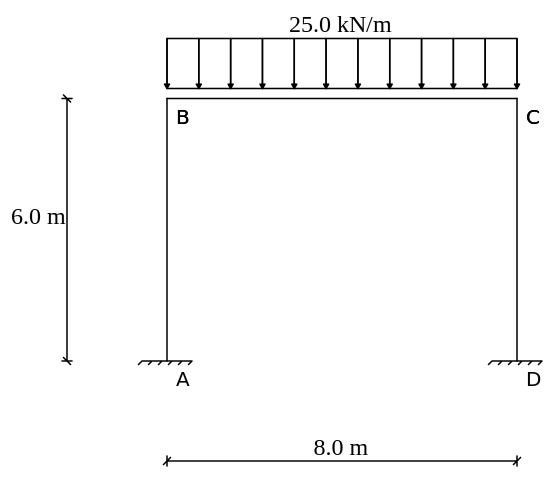
\includegraphics[scale=0.75]{%
                            bm_figures/turtle_figures/bmfr04_turtle.pdf}
    \centering
    \caption{Problem 1: Loading, geometry and supports}
    \label{fig:bmfr04_turtle}
\end{figure}
\lstinputlisting{input_files/bmfr04_input.dat}
\lstinputlisting{output_files/bmfr04_output.dat}
% Deformed
\begin{figure}[!htb]
    \includegraphics[width=\textwidth, keepaspectratio]{%
                     bm_figures/vtk_figures/bmfr04_deformed.pdf}
    \centering
    \caption{FR2, Load Case 1: Deformed Shape}
    \label{fig:bmfr04_deformed}
\end{figure}
% Axial
\begin{figure}[!htb]
    \includegraphics[width=\textwidth, keepaspectratio]{%
                     bm_figures/vtk_figures/bmfr04_axial.pdf}
    \centering
    \caption{FR2, Load Case 1: Axial Force Diagram}
    \label{fig:bmfr04_shear}
\end{figure}
% Shear
\begin{figure}[!htb]
    \includegraphics[width=\textwidth, keepaspectratio]{%
                     bm_figures/vtk_figures/bmfr04_shear.pdf}
    \centering
    \caption{FR2, Load Case 1: Shear Force Diagram}
    \label{fig:bmfr04_shear}
\end{figure}
% Moment
\begin{figure}[!htb]
    \includegraphics[width=\textwidth, keepaspectratio]{%
                     bm_figures/vtk_figures/bmfr04_moment.pdf}
    \centering
    \caption{FR2, Load Case 1: Bending Moment Diagram}
    \label{fig:bmfr04_moment}
\end{figure}
% Error
\begin{table}[h!]
\centering
\begin{tabular}{ c| c c c c }
    & Exact Expression & Exact Value & Computed Value & \% RE \\ \hline \\
    $M_A=M_D$   & $\dfrac{\omega l^2}{12(k+2)}$ &  0.54779E+02 & 0.54779E+02 & 0.0\% \\ \\
    $M_B=M_C$   & $-2M_A$ &  -0.10956E+03 & -0.10956E+03 & 0.0\% \\ \\
    $M_{max}$   & $\dfrac{\omega l^2}{8} + M_B$ &  0.90442E+02 & 0.90442E+02 & 0.0\% \\ \\
    $V_A=V_D$   & $\dfrac{\omega l}{2}$ &  0.10000E+03 & 0.10000E+03 & 0.0\% \\ \\
    $H_A=H_D$   & $\dfrac{3M_A}{h}$ &  0.27389E+02 & 0.27389E+03 & 0.0\% \\ \\
\end{tabular}
\end{table}

%
% LOAD CASE 2
%
\clearpage
\subsubsection{Load Case 2}
\begin{figure}[h]
    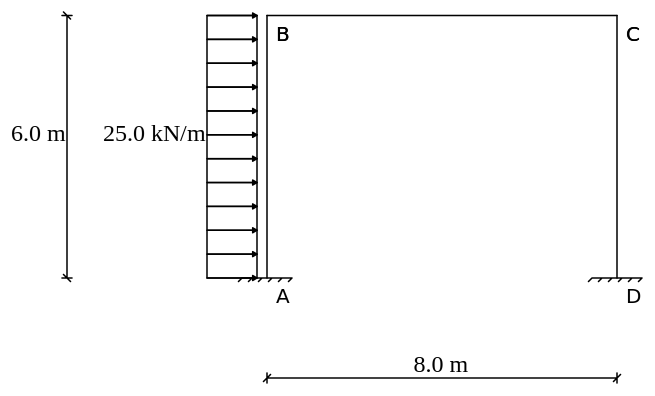
\includegraphics[scale=0.75]{%
                            bm_figures/turtle_figures/bmfr05_turtle.pdf}
    \centering
    \caption{Problem 1: Loading, geometry and supports}
    \label{fig:bmfr05_turtle}
\end{figure}
\lstinputlisting{input_files/bmfr05_input.dat}
\lstinputlisting{output_files/bmfr05_output.dat}
% Deformed
\begin{figure}[!htb]
    \includegraphics[width=\textwidth, keepaspectratio]{%
                     bm_figures/vtk_figures/bmfr05_deformed.pdf}
    \centering
    \caption{FR2, Load Case 2: Deformed Shape}
    \label{fig:bmfr05_deformed}
\end{figure}
% Axial
\begin{figure}[!htb]
    \includegraphics[width=\textwidth, keepaspectratio]{%
                     bm_figures/vtk_figures/bmfr05_axial.pdf}
    \centering
    \caption{FR2, Load Case 2: Axial Force Diagram}
    \label{fig:bmfr05_shear}
\end{figure}
% Shear
\begin{figure}[!htb]
    \includegraphics[width=\textwidth, keepaspectratio]{%
                     bm_figures/vtk_figures/bmfr05_shear.pdf}
    \centering
    \caption{FR2, Load Case 2: Shear Force Diagram}
    \label{fig:bmfr05_shear}
\end{figure}
% Moment
\begin{figure}[!htb]
    \includegraphics[width=\textwidth, keepaspectratio]{%
                     bm_figures/vtk_figures/bmfr05_moment.pdf}
    \centering
    \caption{FR2, Load Case 2: Bending Moment Diagram}
    \label{fig:bmfr05_moment}
\end{figure}
% Error
\begin{table}[h!]
\centering
\begin{tabular}{ c| c c c c }
    & Exact Expression & Exact Value & Computed Value & \% RE \\ \hline \\
    $M_A$   & $\dfrac{\omega h^2}{4}[-\dfrac{k+3}{6(k+2)}-\dfrac{4k+1}{6k+1}]$ & %
                               -0.22372E+03 & -0.22372E+03 & 0.0\% \\ \\
    $M_D$   & $\dfrac{\omega h^2}{4}[-\dfrac{k+3}{6(k+2)}+\dfrac{4k+1}{6k+1}]$ & %
                                0.11790E+03 &  0.11790E+03 & 0.0\% \\ \\
    $M_B$   & $\dfrac{\omega h^2}{4}[-\dfrac{k}{6(k+2)}+\dfrac{2k}{6k+1}]$ & %
                                0.47504E+02 &  0.47504E+02 & 0.0\% \\ \\
    $M_C$   & $\dfrac{\omega h^2}{4}[-\dfrac{k}{6(k+2)}-\dfrac{2k}{6k+1}]$ & %
                               -0.60878E+02 &  0.60878E+02 & 0.0\% \\ \\
    $H_D$   & $\omega h \dfrac{2k+3}{8(k+2}$ & -0.29797E+02 & -0.29797E+02 & 0.0\% \\ \\
    $H_A$   & $-(\omega h-H_D)$ & -0.12020E+03 & -0.12020E+03 & 0.0\% \\ \\
\end{tabular}
\end{table}

%
% LOAD CASE 3
%
\clearpage
\subsubsection{Load Case 3}
\begin{figure}[h]
    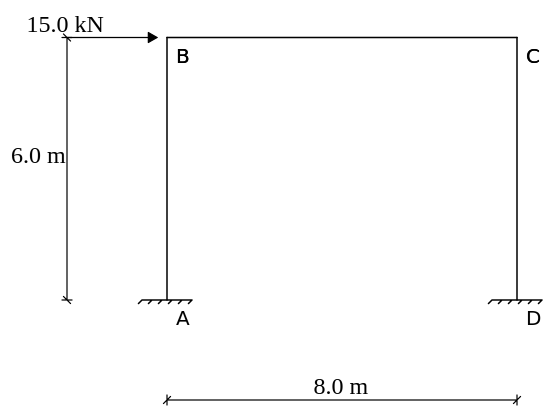
\includegraphics[scale=0.75]{%
                            bm_figures/turtle_figures/bmfr06_turtle.pdf}
    \centering
    \caption{Problem 1: Loading, geometry and supports}
    \label{fig:bmfr06_turtle}
\end{figure}
\lstinputlisting{input_files/bmfr06_input.dat}
\lstinputlisting{output_files/bmfr06_output.dat}
% Deformed
\begin{figure}[!htb]
    \includegraphics[width=\textwidth, keepaspectratio]{%
                     bm_figures/vtk_figures/bmfr06_deformed.pdf}
    \centering
    \caption{FR2, Load Case 3: Deformed Shape}
    \label{fig:bmfr06_deformed}
\end{figure}
% Axial
\begin{figure}[!htb]
    \includegraphics[width=\textwidth, keepaspectratio]{%
                     bm_figures/vtk_figures/bmfr06_axial.pdf}
    \centering
    \caption{FR2, Load Case 3: Axial Force Diagram}
    \label{fig:bmfr06_shear}
\end{figure}
% Shear
\begin{figure}[!htb]
    \includegraphics[width=\textwidth, keepaspectratio]{%
                     bm_figures/vtk_figures/bmfr06_shear.pdf}
    \centering
    \caption{FR2, Load Case 3: Shear Force Diagram}
    \label{fig:bmfr06_shear}
\end{figure}
% Moment
\begin{figure}[!htb]
    \includegraphics[width=\textwidth, keepaspectratio]{%
                     bm_figures/vtk_figures/bmfr06_moment.pdf}
    \centering
    \caption{FR2, Load Case 3: Bending Moment Diagram}
    \label{fig:bmfr06_moment}
\end{figure}
% Error
\begin{table}[h!]
\centering
\begin{tabular}{ c| c c c c }
    & Exact Expression & Exact Value & Computed Value & \% RE \\ \hline \\
    $M_D=-M_A$  & $\dfrac{Ph}{2}[-\dfrac{3k+1}{6k+1)}$ 0.95809E+02 & 0.95809E+02 & 0.0\% \\ \\
    $M_B=-M_C$  & $\dfrac{Ph}{2}[\dfrac{3k}{6k+1)}$ 0.54191E+02 & 0.54191E+02 & 0.0\% \\ \\
    $V_D=-V_A$  & $\dfrac{2M_B}/{l}$ & 0.13548E+02 & 0.13548E+02 & 0.0\% \\ \\
    $H_D=H_A$   & ${P}/{2}$ & -0.25000E+02 & -0.25000E+02 & 0.0\% \\ \\
\end{tabular}
\end{table}

